\section{A MAC Layer in \mbox{Mote Runner}}
\begin{frame}[fragile]
  \frametitle{Design strategy}
  \begin{itemize}
    \item Mac class behaviours:
    \begin{itemize}
      \item Coordinator -> Beacon enabled, Slotted CSMA/CA
      \item Unassociated -> Handles association with a Coordinator
      \item Associated -> Sends data from upper layer and receives data from Coordinator
    \end{itemize}
    \item Flexibility:
    \begin{itemize}
    	\item State changes are ruled by Mac class through events
    	\item Mac can handle more than one state -> Mac - entities
    	\begin{itemize}
	  \item e.g.: Coordinator - Associated
    	\end{itemize}
    \end{itemize}
  \end{itemize}
\end{frame}

\begin{frame}[fragile]
  \frametitle{The concept}
  \begin{figure}
    \centering
    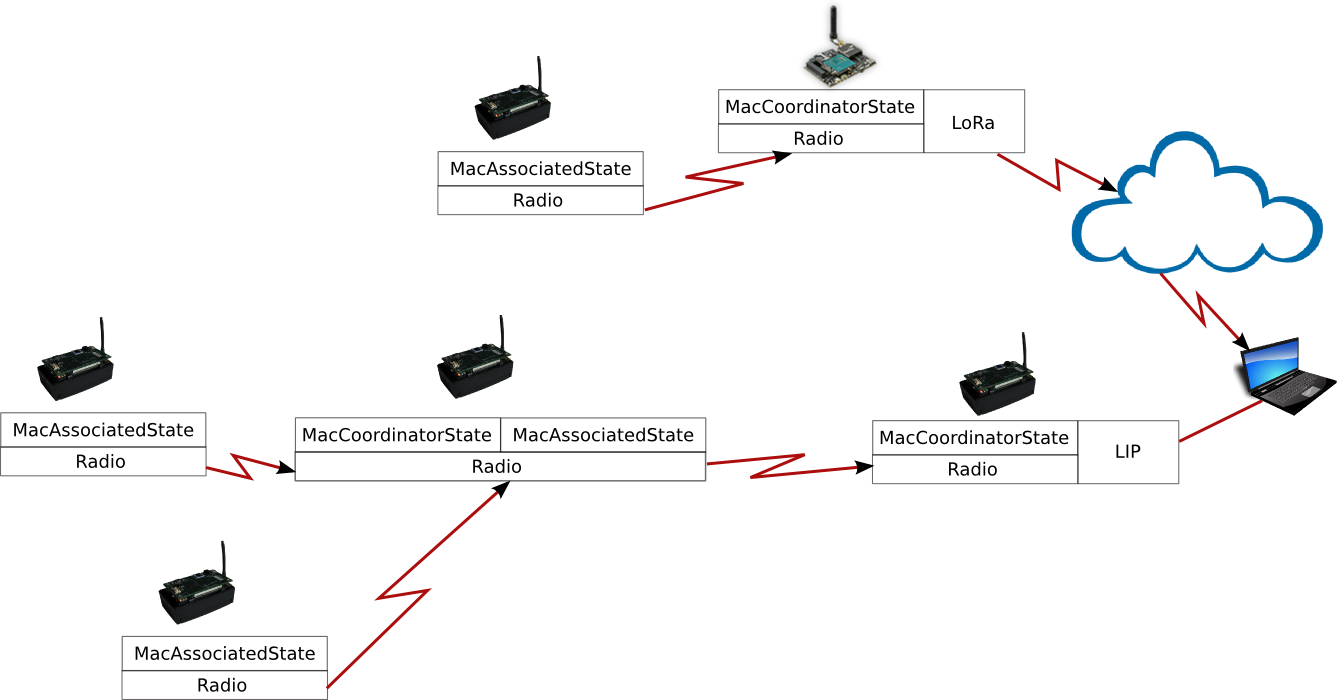
\includegraphics[width=\textwidth]{img/MAClan.png}
  \end{figure}
\end{frame}

\begin{frame}[fragile]
  \frametitle{About the concept}
  \begin{itemize}
    \item Motes have to be subdivided into PANs
    \begin{itemize}
    	\item Every PAN as a PAN Id
    	\item Every mote has a unique short address (SADDR) inside the PAN
    \end{itemize}
    \item To obtain the SADDR the mote has to require association with the PAN coordinator
    \item To grant communication between motes it's needed synchronization
    \begin{itemize}
      \item Beacon + Superframe
    \end{itemize}
    \item The adopted procedures follow 802.15.4 standard
  \end{itemize}

\end{frame}

\begin{frame}[fragile]
  \frametitle{Association}
  \begin{figure}
    \centering
    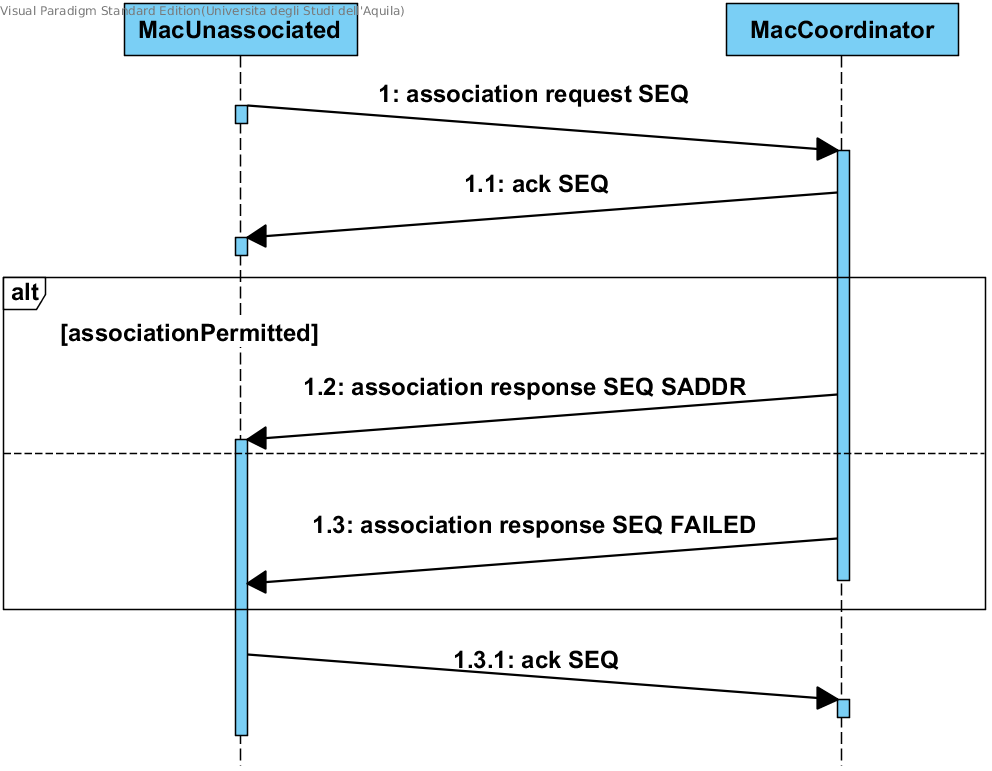
\includegraphics[width=.8\textwidth]{img/Association.png}
  \end{figure}
\end{frame}

\begin{frame}[fragile]
  \frametitle{Data indirect}
  \vspace{-2.7em}
  \begin{figure}
    \centering
    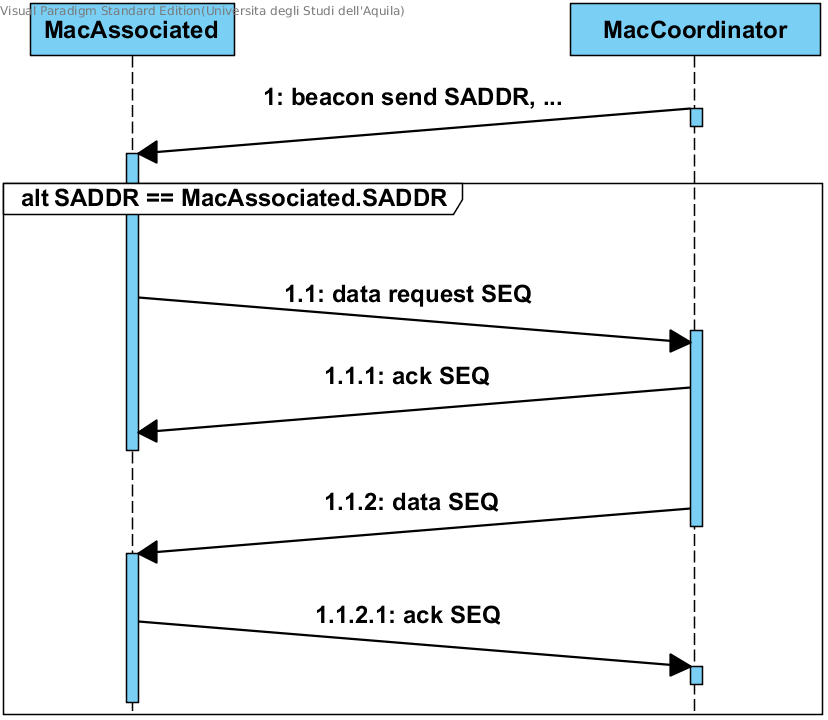
\includegraphics[width=.7\textwidth]{img/DataRequest.png}
  \end{figure}
\end{frame}

\begin{frame}[fragile]
  \frametitle{Timing with beacon}
  \begin{itemize}
    \item It grants synchronization between mote and coordinator
    \item Realized with a timer and scheduled events
  \end{itemize}
  \begin{figure}
    \centering
    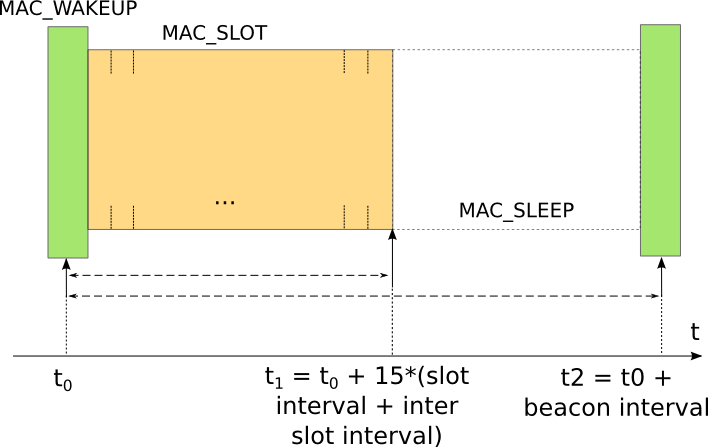
\includegraphics[width=.7\textwidth]{img/MAC_STATES.png}
  \end{figure}
\end{frame}

\begin{frame}[fragile]
  \frametitle{Beacon}
  \begin{columns}
    \begin{column}{.58\linewidth}
      \begin{itemize}
      	\item Superframe Specification:
      	\begin{itemize}
	  \item Beacon Order -> BO
	  \item Superframe Order -> SO
	  \item Association permitted
      	\end{itemize}
      \end{itemize}
    \end{column}
    \hfill
    \begin{column}{.4\linewidth}
      \begin{figure}
	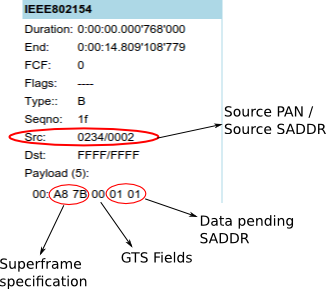
\includegraphics[width=\textwidth]{img/beacon.png}
      \end{figure}
    \end{column}
  \end{columns}
  \vfill
  $$\text{Beacon Interval} = \frac{60sym \cdot n.Slot \cdot 2^{BO}}{20\text{kbps}}$$
  $$\text{Superframe Duration} = \frac{60sym \cdot n.Slot \cdot 2^SO}{20\text{kbps}}$$
\end{frame}


\begin{frame}[fragile]
  \frametitle{Mac Coordinator Behaviour}
  \vspace{-2.7em}
  \begin{figure}
    \centering
    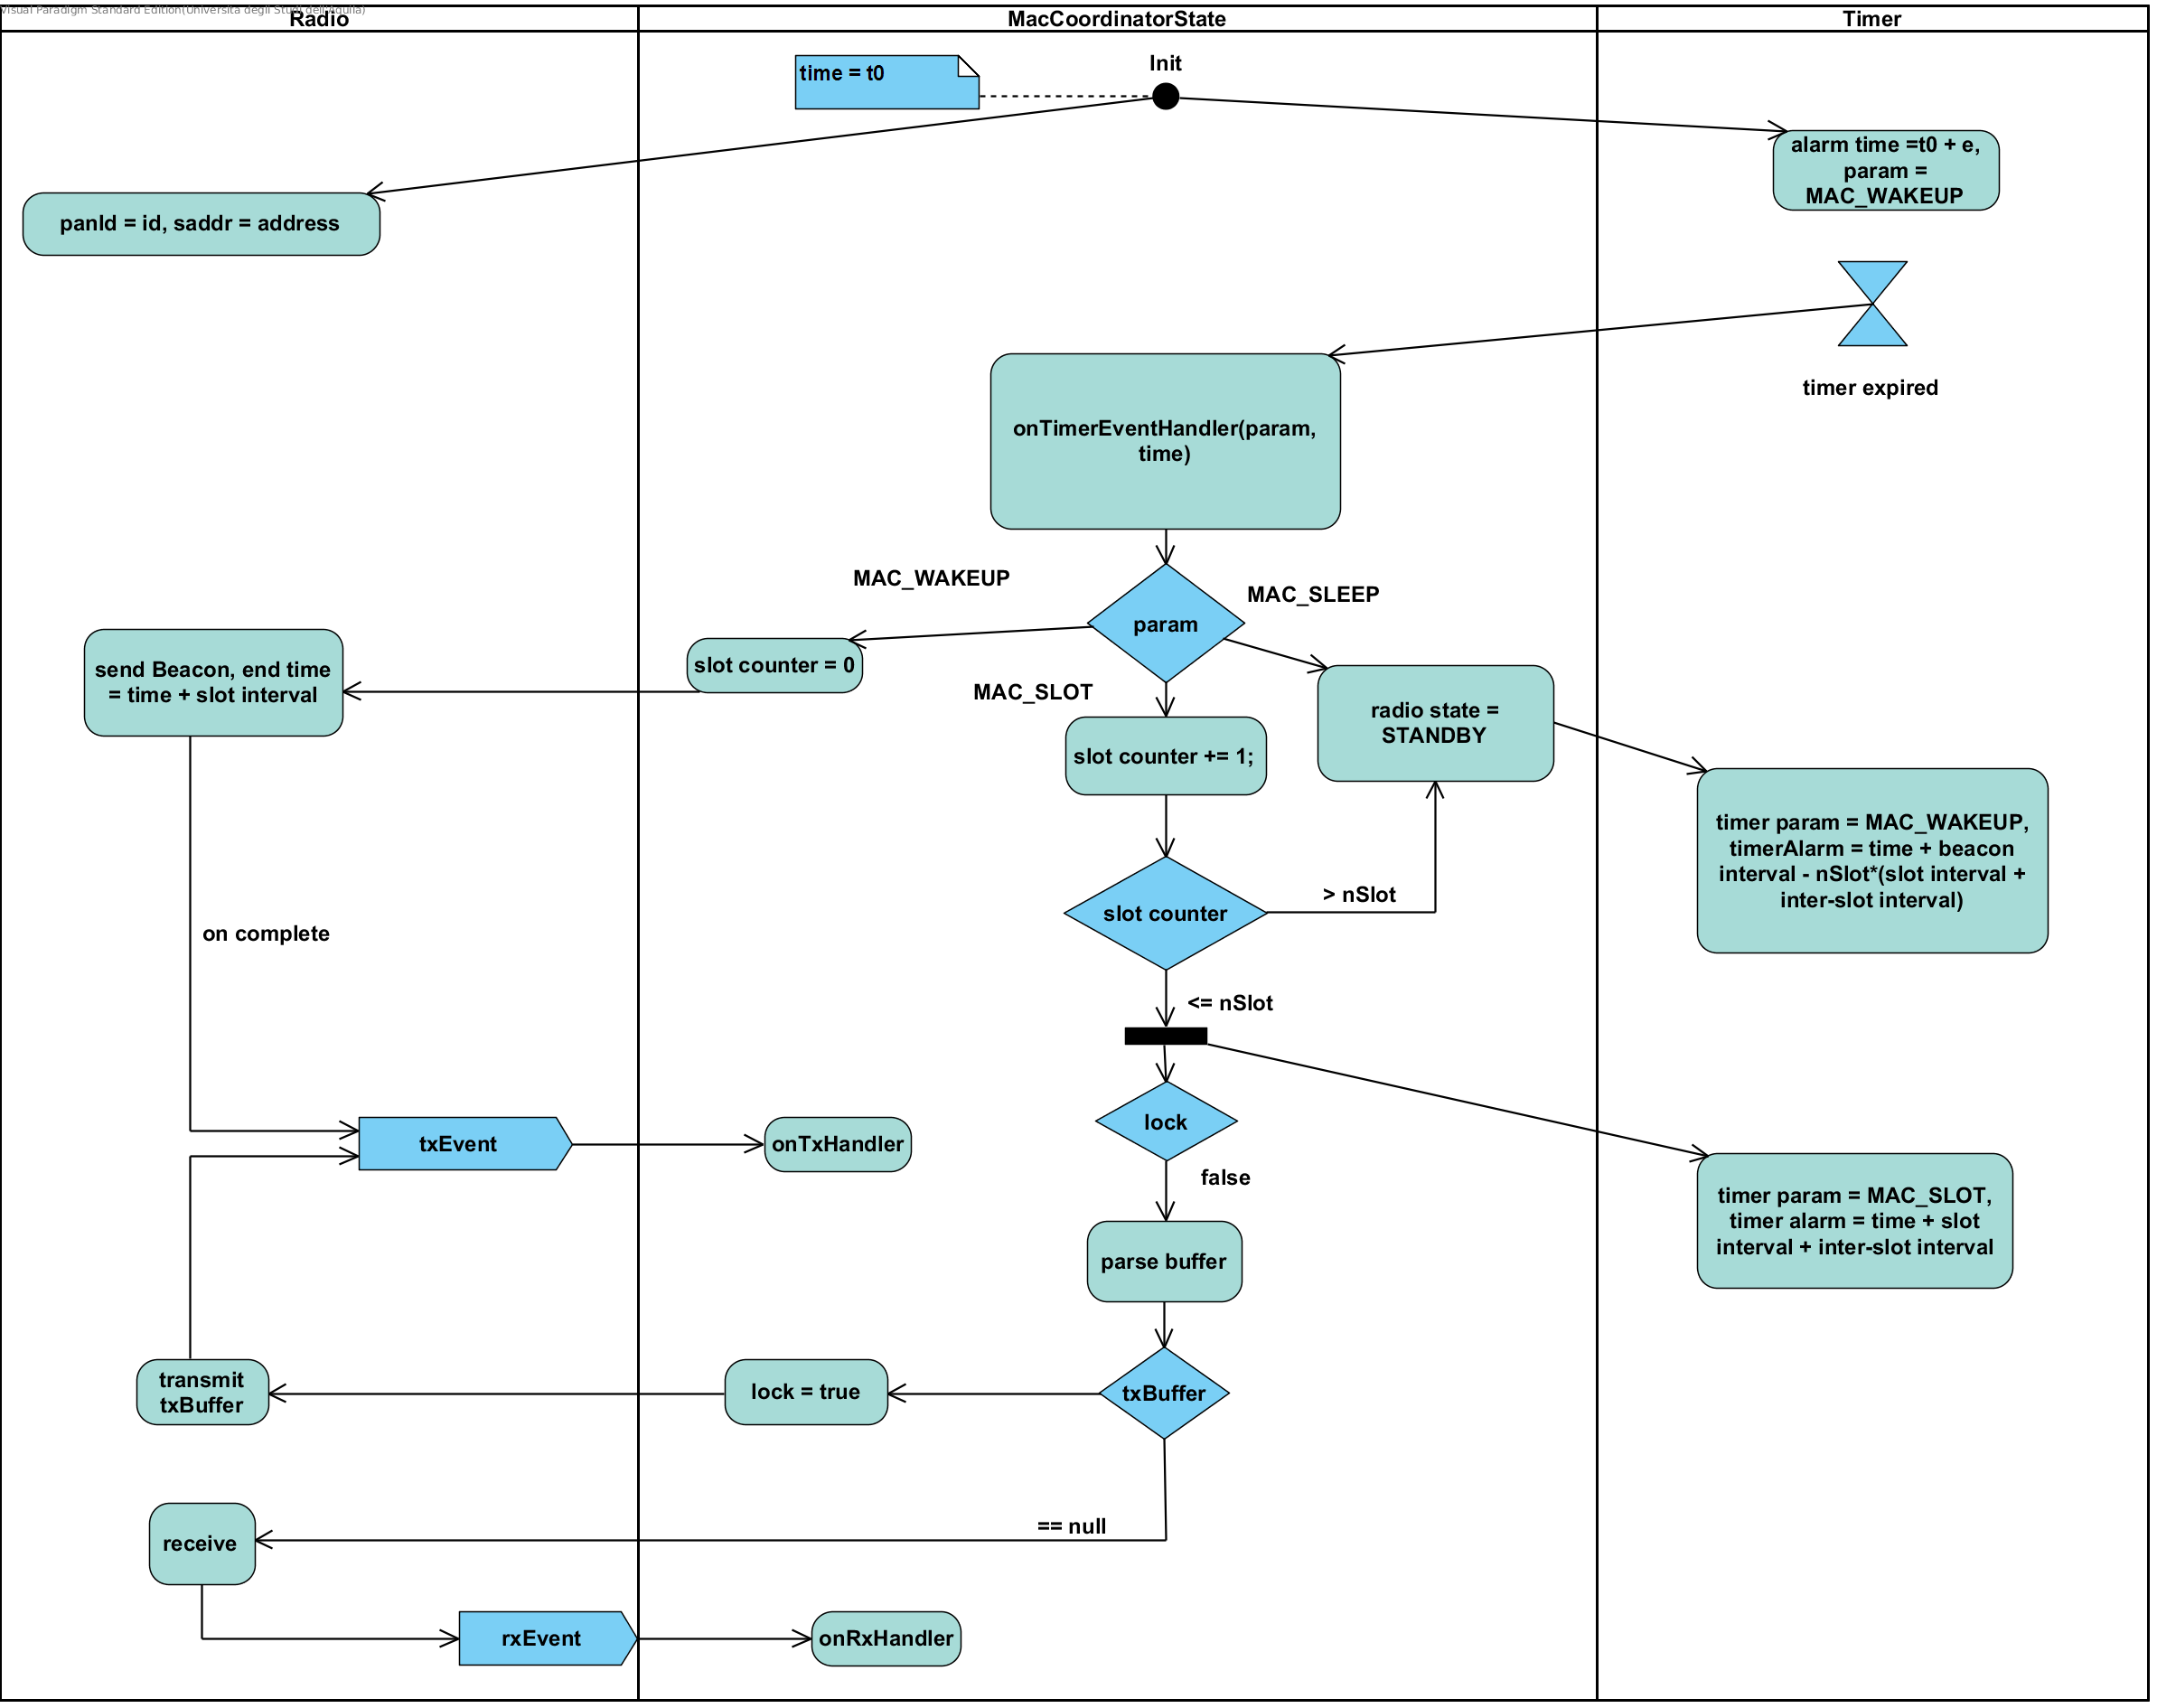
\includegraphics[width=.99\textwidth]{img/MAC_COORDINATOR.png}
  \end{figure}
\end{frame}

\begin{frame}[fragile]
  \frametitle{Example}
  \vspace{-2em}
  The node associates with coordinator, then responds to beacon pending list and gets data.
  \begin{figure}
    \centering
    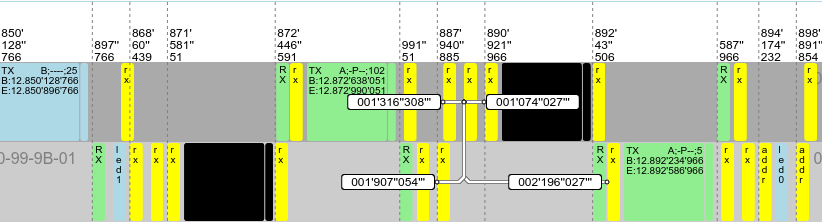
\includegraphics[width=\textwidth]{img/associazione.png}
  \end{figure}
  \begin{figure}
    \centering
    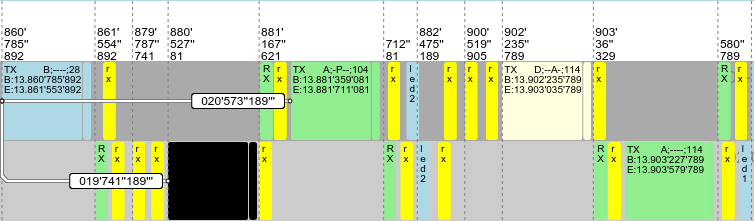
\includegraphics[width=\textwidth]{img/dataIndirect.png}
  \end{figure}
\end{frame}


